\documentclass[a4paper]{article}

%% Language and font encodings
\usepackage[english]{babel}
\usepackage[utf8x]{inputenc}
\usepackage[T1]{fontenc}

%% Sets page size and margins
\usepackage[a4paper,top=3cm,bottom=2cm,left=3cm,right=3cm,marginparwidth=1.75cm]{geometry}

%% Useful packages
\usepackage{amsmath}
\usepackage{graphicx}
\usepackage[colorinlistoftodos]{todonotes}
\usepackage[colorlinks=true, allcolors=blue]{hyperref}
\usepackage{float}


\title{Benchmarking P2C for HPC}
\author{Joseph Anthony C. Hermocilla}

\begin{document}
\maketitle

\begin{abstract}
We report some benchmarking results of the Peak-Two(P2C) Cloud for High-Performance Computing(HPC) using the NAS Parallel Benchmarks (NPB).
\end{abstract}

\section{Introduction}

In order to evaluate the performance of the P2C\cite{hermocilla-p2c-ncite2014} for HPC, NPB\footnote{https://www.nas.nasa.gov/publications/npb.html} version 3.3.1 was run on a 16-node MPI cluster provisioned using vcluster\footnote{http://srg.ics.uplb.edu.ph/projects/peak-two-cloud/peak-two-cloud-resources/deployinganmpiclusterusingvcluster}.

NPB consists of a set of programs that implements different computational approaches associated with Computational Fluid Dynamics(CFD). These programs represent the types of applications that are run in supercomputers and HPC clusters. In running the benchmark, classes A and B were used for each program. Different classes have different problem sizes and parameters which result to different measurements.

\section{Results}

\subsection{Conjugate Gradient}

\begin{figure}[H]
\centering
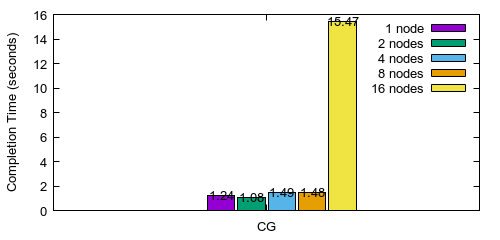
\includegraphics[width=0.8\textwidth]{figures/CGvA.png}
\caption{\label{fig:CGvA}}
\end{figure}

\begin{figure}[H]
\centering
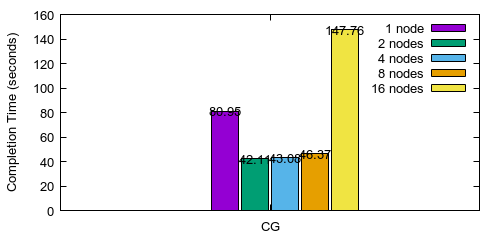
\includegraphics[width=0.8\textwidth]{figures/CGvB.png}
\caption{\label{fig:CGvB}}
\end{figure}

\subsection{Embarassingly Parallel}

\begin{figure}[H]
\centering
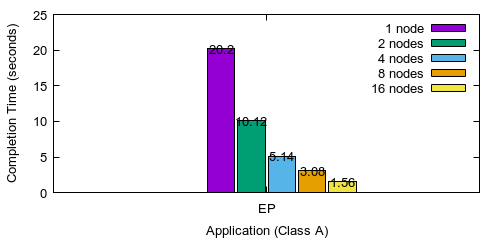
\includegraphics[width=0.8\textwidth]{figures/EPvA.png}
\caption{\label{fig:EPvA}}
\end{figure}

\begin{figure}[H]
\centering
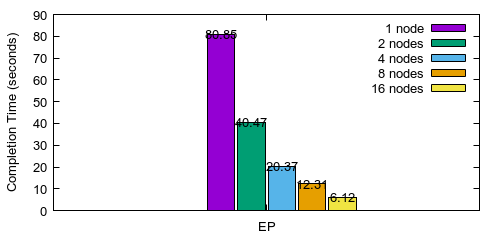
\includegraphics[width=0.8\textwidth]{figures/EPvB.png}
\caption{\label{fig:EPvB}}
\end{figure}


\subsection{Fourier Transform}

\begin{figure}[H]
\centering
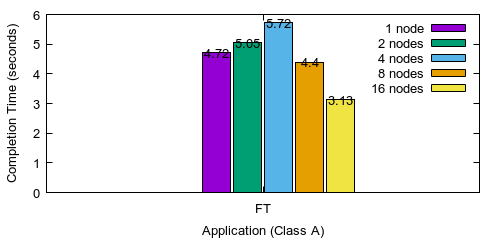
\includegraphics[width=0.8\textwidth]{figures/FTvA.png}
\caption{\label{fig:FTvA}}
\end{figure}

\begin{figure}[H]
\centering
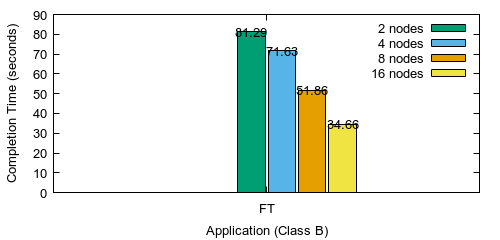
\includegraphics[width=0.8\textwidth]{figures/FTvB.png}
\caption{\label{fig:FTvB}}
\end{figure}

\subsection{Integer Sort}

\begin{figure}[H]
\centering
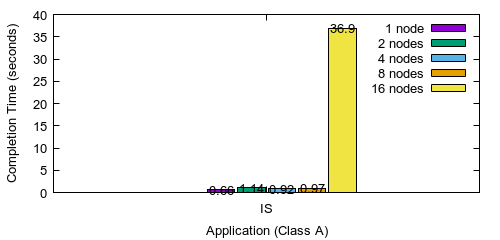
\includegraphics[width=0.8\textwidth]{figures/ISvA.png}
\caption{\label{fig:ISvA}}
\end{figure}

\begin{figure}[H]
\centering
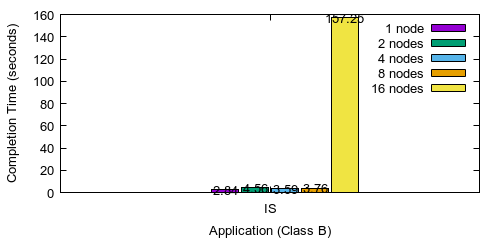
\includegraphics[width=0.8\textwidth]{figures/ISvB.png}
\caption{\label{fig:ISvB}}
\end{figure}

\subsection{Lower-Upper Gauss-Seidel Solver}

\begin{figure}[H]
\centering
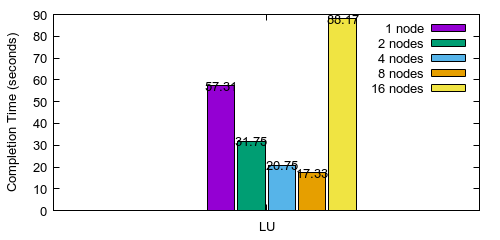
\includegraphics[width=0.8\textwidth]{figures/LUvA.png}
\caption{\label{fig:LUvA}}
\end{figure}

\begin{figure}[H]
\centering
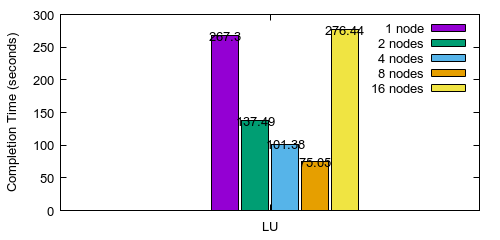
\includegraphics[width=0.8\textwidth]{figures/LUvB.png}
\caption{\label{fig:LUvB}}
\end{figure}

\subsection{Multi-Grid}

\begin{figure}[H]
\centering
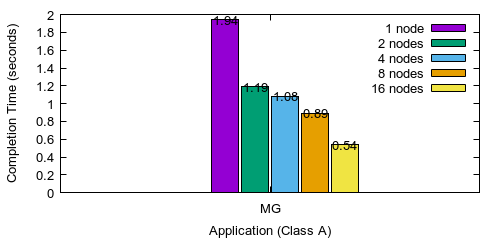
\includegraphics[width=0.8\textwidth]{figures/MGvA.png}
\caption{\label{fig:MGvA}}
\end{figure}

\begin{figure}[H]
\centering
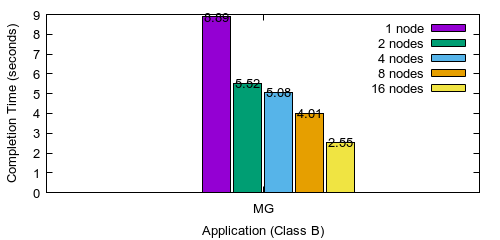
\includegraphics[width=0.8\textwidth]{figures/MGvB.png}
\caption{\label{fig:MGvB}}
\end{figure}

\bibliographystyle{abbrv}
\bibliography{p2c-benchmark}

\end{document}